\documentclass{article}
\usepackage{amsmath,amssymb}
\usepackage{graphicx}
\usepackage{CJK}
\author{张奇 PB19000093}
\title{数值分析 code5 说明文档}
\begin{document}
\begin{CJK}{UTF8}{gbsn}
	\maketitle
	\section{问题描述}
		本次实验要求,用复化的Simpson积分公式和梯形积分公式结算下面积分,
		\[\int_{0}^{4} \sin x d x . \]
		其中复化的区间个数按照$n=2^k, k=1,\cdots,12.$来计算,并且利用 
		$\mbox{order} = \dfrac{\log(\varepsilon_0/\varepsilon_1)}{\log(N_1/N_0)}$来计算收敛阶,以固定的格式输出。
	\section{算法原理}
		本实验只需实现计算Simpson复化积分和梯形积分即可,若选取的节点为$\{x_i\}_{i=0}^n$,那么梯形积分公式为
		\[\int_{x_0}^{x_n} f \approxeq \sum_{i=1}^{n} h_i (f(x_{i-1}) + f(x_{i}))/2, h_i = x_i-x_{i-1}.\]
		以及Simpson积分公式,
		\[\int_{x_0}^{x_n} f \approxeq \sum_{i=1}^{n} h_i (f(x_{i-1})/6 + f( \frac{x_{i-1}+x_i}{2} )2/3 + f(x_{i})/6), h_i = x_i-x_{i-1}.\]
	\section{编程实现}
	设计两个函数,求解,
	\begin{itemize}
		\item  double splined\_line(double f(double), double l, double r, int n)
		\item double splined\_simpson(double f(double), double l, double r, int n)
	\end{itemize}
	\section{编译环境}
	\begin{itemize}
		\item Ubuntu20.4LTS, g++9.4.0
		\item 编译命令+运行:./run main
	\end{itemize}
	\section{结果分析}
	\begin{figure}[hbpt]
		\centering
		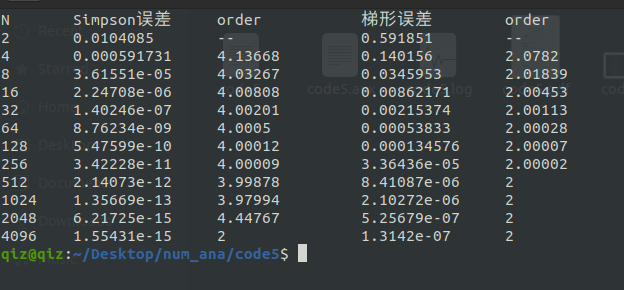
\includegraphics[width = 0.6\linewidth]{code5.png}
		\caption{实验结果}
	\end{figure}
	\paragraph{分析}
	\begin{itemize}
		\item Simpson积分收敛要比梯形积分要好。
		\item Simpson积分的收敛阶会出现不稳定情况。
	\end{itemize}
\end{CJK}
\end{document}